%
\begin{isabellebody}%
\setisabellecontext{Introduction}%
%
\isadelimdocument
%
\endisadelimdocument
%
\isatagdocument
%
\isamarkupchapter{A Gentle Introduction to TESL%
}
\isamarkuptrue%
%
\endisatagdocument
{\isafolddocument}%
%
\isadelimdocument
%
\endisadelimdocument
%
\isadelimtheory
%
\endisadelimtheory
%
\isatagtheory
%
\endisatagtheory
{\isafoldtheory}%
%
\isadelimtheory
%
\endisadelimtheory
%
\isadelimdocument
%
\endisadelimdocument
%
\isatagdocument
%
\isamarkupsection{Context%
}
\isamarkuptrue%
%
\endisatagdocument
{\isafolddocument}%
%
\isadelimdocument
%
\endisadelimdocument
%
\begin{isamarkuptext}%
The design of complex systems involves different formalisms for modeling their different parts or 
aspects. The global model of a system may therefore consist of a coordination of concurrent 
sub-models that use different paradigms such as differential equations, state machines, 
synchronous data-flow networks, 
discrete event models and so on, as illustrated in \autoref{fig:het-timed-system}. 
This raises the interest in architectural composition languages 
that allow for ``bolting the respective sub-models together'', along their various interfaces, and 
specifying the various ways of collaboration and coordination~\cite{nguyenvan:hal-01583815}.

We are interested in languages that allow for specifying the timed coordination of subsystems by 
addressing the following conceptual issues:

%
\begin{itemize}%
\item events may occur in different sub-systems at unrelated times, leading to \emph{polychronous} systems, 
which do not necessarily have a common base clock,

\item the behavior of the sub-systems is observed only at a series of discrete instants, and time 
coordination has to take this \emph{discretization} into account,

\item the instants at which a system is observed may be arbitrary and should not change its behavior 
(\emph{stuttering invariance}),

\item coordination between subsystems involves causality, so the occurrence of an event may enforce 
the occurrence of other events, possibly after a certain duration has elapsed or an event has 
occurred a given number of times,

\item the domain of time (discrete, rational, continuous. . . ) may be different in the subsystems, 
leading to \emph{polytimed} systems,

\item the time frames of different sub-systems may be related (for instance, time in a GPS satellite 
and in a GPS receiver on Earth are related although they are not the same).%
\end{itemize}%
\end{isamarkuptext}\isamarkuptrue%
%
\begin{isamarkuptext}%
\begin{figure}[htbp]
 \centering
 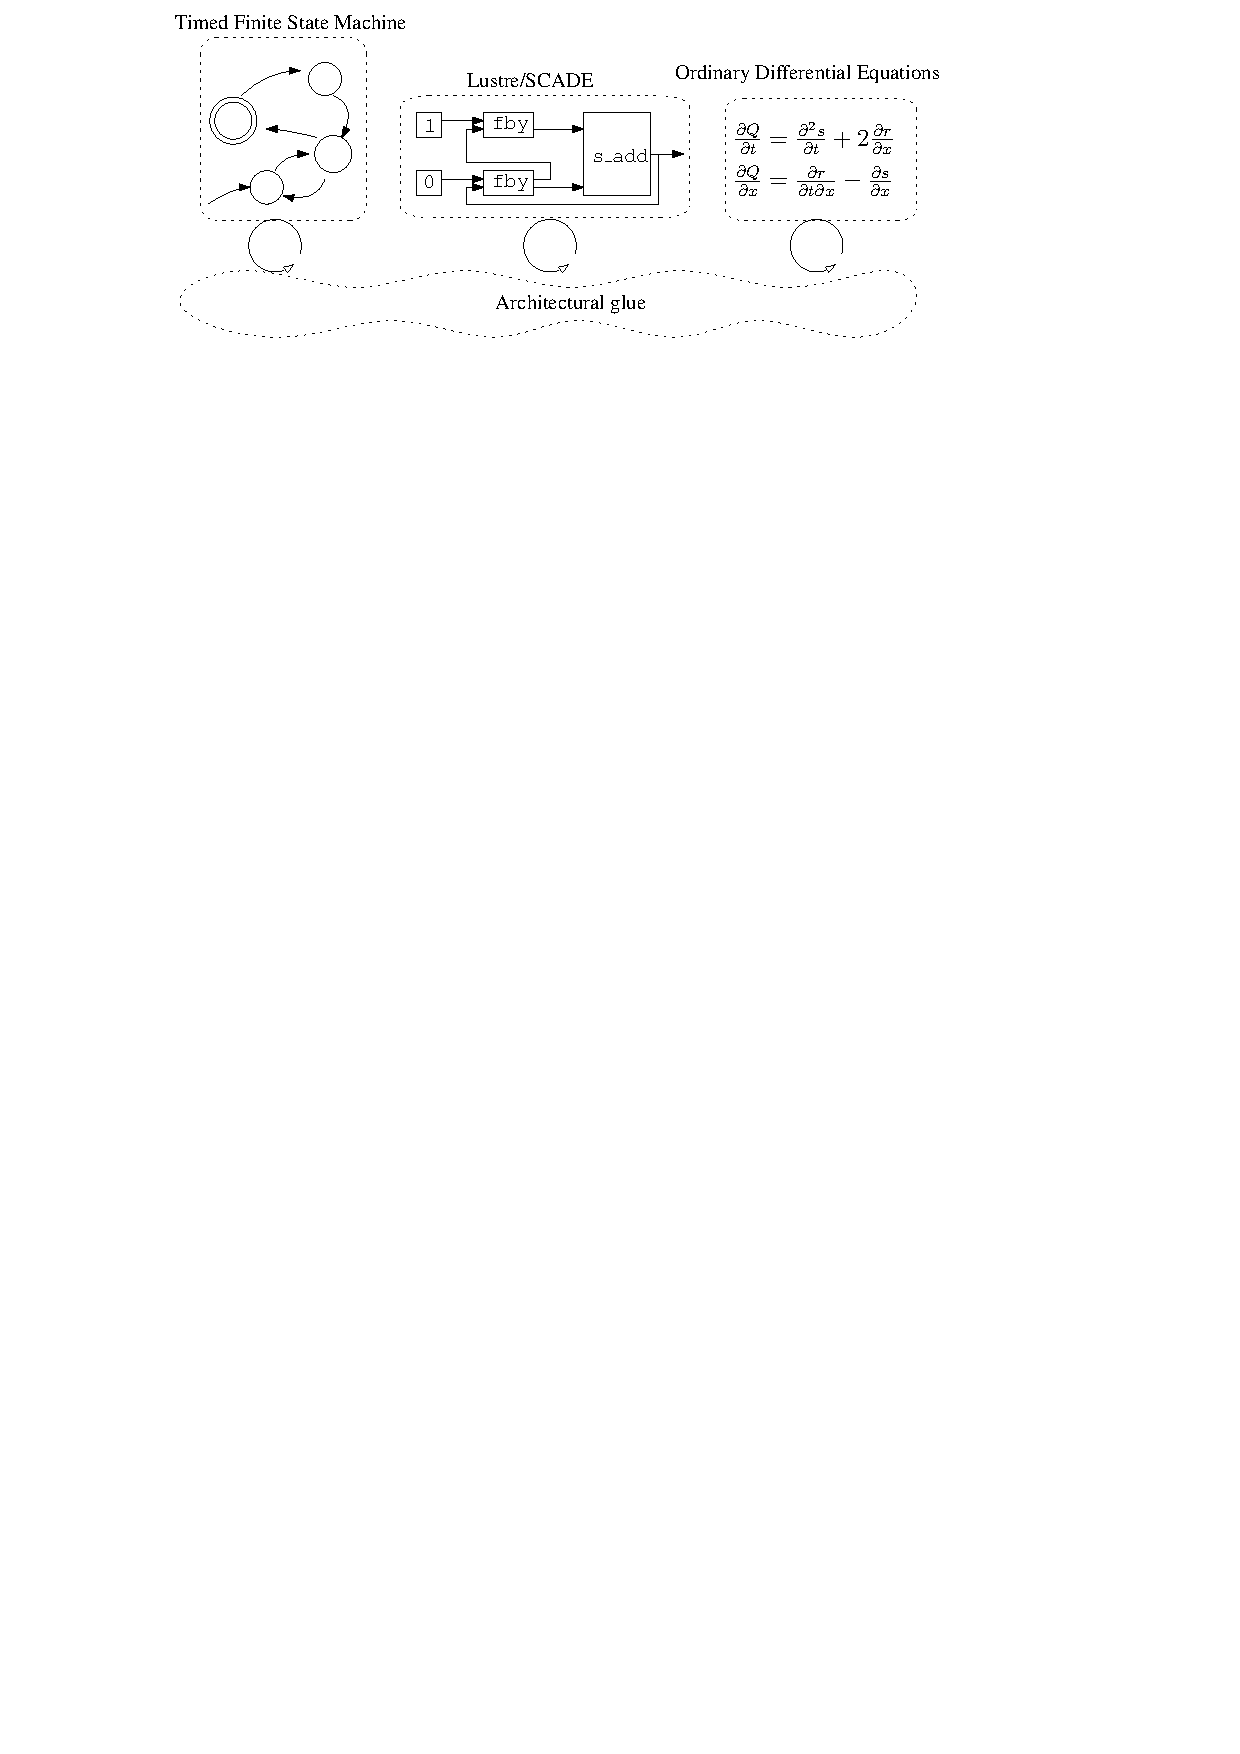
\includegraphics{glue.pdf}
 \caption{A Heterogeneous Timed System Model}
 \label{fig:het-timed-system}
\end{figure}%
\end{isamarkuptext}\isamarkuptrue%
%
\begin{isamarkuptext}%
In order to tackle the heterogeneous nature of the subsystems, we abstract their behavior as clocks. 
Each clock models an event, i.e., something that can occur or not at a given time. This time is measured 
in a time frame associated with each clock, and the nature of time (integer, rational, real, or any 
type with a linear order) is specific to each clock. 
When the event associated with a clock occurs, the clock ticks. In order to support any kind of 
behavior for the subsystems, we are only interested in specifying what we can observe at a series 
of discrete instants. There are two constraints on observations: a clock may tick only at an 
observation instant, and the time on any clock cannot decrease from an instant to the next one. 
However, it is always possible to add arbitrary observation instants, which allows for stuttering 
and modular composition of systems. 
As a consequence, the key concept of our setting is the notion of a clock-indexed Kripke model: 
\isa{{\isasymSigma}\isactrlsup {\isasyminfinity}\ {\isacharequal}\ {\isasymnat}\ {\isasymrightarrow}\ {\isasymK}\ {\isasymrightarrow}\ {\isacharparenleft}{\isasymbool}\ {\isasymtimes}\ {\isasymT}{\isacharparenright}}, where \isa{{\isasymK}} is an enumerable set of clocks, \isa{{\isasymbool}} 
is the set of booleans – used to  indicate that a clock ticks at a given instant – and \isa{{\isasymT}} 
is a universal metric time space for which we only assume that it is large enough to contain all 
individual time spaces of clocks and that it is ordered by some linear ordering \isa{{\isacharparenleft}{\isasymle}\isactrlsub {\isasymT}{\isacharparenright}}.%
\end{isamarkuptext}\isamarkuptrue%
%
\begin{isamarkuptext}%
The elements of \isa{{\isasymSigma}\isactrlsup {\isasyminfinity}} are called runs. A specification language is a set of 
  operators that constrains the set of possible monotonic runs. Specifications are composed by 
  intersecting the denoted run sets of constraint operators.
  Consequently, such specification languages do not limit the number of clocks used to model a 
  system (as long as it is finite) and it is always possible to add clocks to a specification. 
  Moreover, they are \emph{compositional} by construction since the composition of specifications 
  consists of the conjunction of their constraints.%
\end{isamarkuptext}\isamarkuptrue%
%
\begin{isamarkuptext}%
This work provides the following contributions:

%
\begin{itemize}%
\item defining the non-trivial language \isa{TESL\isactrlsup {\isacharasterisk}} in terms of clock-indexed Kripke models, 

\item proving that this denotational semantics is stuttering invariant,

\item defining an adapted form of symbolic primitives and presenting the set of operational 
semantic rules,

\item presenting formal proofs for soundness, completeness, and progress of the latter.%
\end{itemize}%
\end{isamarkuptext}\isamarkuptrue%
%
\isadelimdocument
%
\endisadelimdocument
%
\isatagdocument
%
\isamarkupsection{The TESL Language%
}
\isamarkuptrue%
%
\endisatagdocument
{\isafolddocument}%
%
\isadelimdocument
%
\endisadelimdocument
%
\begin{isamarkuptext}%
The TESL language \cite{BouJacHarPro2014MEMOCODE} was initially designed to coordinate the
  execution of heterogeneous components during the simulation of a system. We define here a minimal
  kernel of operators that will form the basis of a family of specification languages, including the
  original TESL language, which is described at \url{http://wdi.supelec.fr/software/TESL/}.%
\end{isamarkuptext}\isamarkuptrue%
%
\isadelimdocument
%
\endisadelimdocument
%
\isatagdocument
%
\isamarkupsubsection{Instantaneous Causal Operators%
}
\isamarkuptrue%
%
\endisatagdocument
{\isafolddocument}%
%
\isadelimdocument
%
\endisadelimdocument
%
\begin{isamarkuptext}%
TESL has operators to deal with instantaneous causality, i.e., to react to an event occurrence
in the very same observation instant.

%
\begin{itemize}%
\item \isatt{c1\ implies\ c2} means that at any instant where \isatt{c1} ticks, \isatt{c2} has to tick too.

\item \isatt{c1\ implies\ not\ c2} means that at any instant where \isatt{c1} ticks, \isatt{c2} cannot tick.

\item \isatt{c1\ kills\ c2} means that at any instant where \isatt{c1} ticks, and at any future instant, 
\isatt{c2} cannot tick.%
\end{itemize}%
\end{isamarkuptext}\isamarkuptrue%
%
\isadelimdocument
%
\endisadelimdocument
%
\isatagdocument
%
\isamarkupsubsection{Temporal Operators%
}
\isamarkuptrue%
%
\endisatagdocument
{\isafolddocument}%
%
\isadelimdocument
%
\endisadelimdocument
%
\begin{isamarkuptext}%
TESL also has chronometric temporal operators that deal with dates and chronometric delays.

%
\begin{itemize}%
\item \isatt{c\ sporadic\ t} means that clock \isatt{c} must have a tick at time \isatt{t} on its own time scale.

\item \isatt{c1\ sporadic\ t\ on\ c2} means that clock \isatt{c1} must have a tick at an instant where the time 
on \isatt{c2} is \isatt{t}.

\item \isatt{c1\ time\ delayed\ by\ d\ on\ m\ implies\ c2} means that every time clock \isatt{c1} ticks, \isatt{c2} must have 
a tick at the first instant where the time on \isatt{m} is \isatt{d} later than it was when \isatt{c1} had ticked.
This means that every tick on \isatt{c1} is followed by a tick on \isatt{c2} after a delay \isatt{d} measured
on the time scale of clock \isatt{m}.

\item \isatt{c1\ time\ delayed{\char`\\}{\char`\<}bowtie{\char`\>}\ by\ d\ on\ m\ implies\ c2} means that every time clock \isatt{c1} ticks, \isatt{c2} must have 
a tick at an instant where the time on \isatt{m} is \isatt{d} later than it was when \isatt{c1} had ticked.
This means that every tick on \isatt{c1} is followed by at least a tick on \isatt{c2} after a delay \isatt{d} 
measured on the time scale of clock \isatt{m}. Contrary to the strict version of \isatt{time\ delayed},
\isatt{c2} may not tick at the first instant at which the delay expires, and it may tick at several
instants, provided that the time on  \isatt{m} is still  \isatt{d} later than it was when \isatt{c1} had ticked.

\item \isatt{time\ relation\ (c1{\char`\,}\ c2)\ in\ R} means that at every instant, the current time on clocks \isatt{c1}
and \isatt{c2} must be in relation \isatt{R}. By default, the time lines of different clocks are 
independent. This operator allows us to link two time lines, for instance to model the fact
that time in a GPS satellite and time in a GPS receiver on Earth are not the same but are 
related. Time being polymorphic in TESL, this can also be used to model the fact that the
angular position on the camshaft of an engine moves twice as fast as the angular position 
on the crankshaft~\footnote{See \url{http://wdi.supelec.fr/software/TESL/GalleryEngine} for more details}. 
We may consider only linear arithmetic relations to restrict the problem to a domain where 
the resolution is decidable.%
\end{itemize}%
\end{isamarkuptext}\isamarkuptrue%
%
\isadelimdocument
%
\endisadelimdocument
%
\isatagdocument
%
\isamarkupsubsection{Asynchronous Operators%
}
\isamarkuptrue%
%
\endisatagdocument
{\isafolddocument}%
%
\isadelimdocument
%
\endisadelimdocument
%
\begin{isamarkuptext}%
The last category of TESL operators allows the specification of asynchronous relations between
event occurrences. They do not specify the precise instants at which ticks have to occur, 
they only put bounds on the set of instants at which they should occur.

%
\begin{itemize}%
\item \isatt{c1\ weakly\ precedes\ c2} means that for each tick on \isatt{c2}, there must be at least one tick
on \isatt{c1} at a previous or at the same instant. This can also be expressed by stating
that at each instant, the number of ticks since the beginning of the run must be lower or 
equal on \isatt{c2} than on \isatt{c1}.

\item \isatt{c1\ strictly\ precedes\ c2} means that for each tick on \isatt{c2}, there must be at least one tick
on \isatt{c1} at a previous instant. This can also be expressed by saying that at each instant, 
the number of ticks on \isatt{c2} from the beginning of the run to this instant, must be lower or 
equal to the number of ticks on \isatt{c1} from the beginning of the run to the previous instant.%
\end{itemize}%
\end{isamarkuptext}\isamarkuptrue%
%
\isadelimtheory
%
\endisadelimtheory
%
\isatagtheory
%
\endisatagtheory
{\isafoldtheory}%
%
\isadelimtheory
%
\endisadelimtheory
%
\end{isabellebody}%
\endinput
%:%file=~/Documents/Recherche/Thesards/2014_Hai_NGUYEN_VAN/Heron_git/reiher2/TESL_Theory/src/Introduction.thy%:%
%:%11=1%:%
%:%41=10%:%
%:%53=12%:%
%:%54=13%:%
%:%55=14%:%
%:%56=15%:%
%:%57=16%:%
%:%58=17%:%
%:%59=18%:%
%:%60=19%:%
%:%62=21%:%
%:%63=22%:%
%:%67=23%:%
%:%68=24%:%
%:%70=25%:%
%:%71=26%:%
%:%73=27%:%
%:%74=28%:%
%:%76=29%:%
%:%77=30%:%
%:%78=31%:%
%:%80=32%:%
%:%81=33%:%
%:%83=34%:%
%:%84=35%:%
%:%89=39%:%
%:%90=40%:%
%:%91=41%:%
%:%92=42%:%
%:%93=43%:%
%:%94=44%:%
%:%98=66%:%
%:%99=67%:%
%:%100=68%:%
%:%101=69%:%
%:%102=70%:%
%:%103=71%:%
%:%104=72%:%
%:%105=73%:%
%:%106=74%:%
%:%107=75%:%
%:%108=76%:%
%:%109=77%:%
%:%110=78%:%
%:%111=79%:%
%:%112=80%:%
%:%116=84%:%
%:%117=85%:%
%:%118=86%:%
%:%119=87%:%
%:%120=88%:%
%:%121=89%:%
%:%122=90%:%
%:%126=94%:%
%:%130=95%:%
%:%132=96%:%
%:%134=97%:%
%:%135=98%:%
%:%137=99%:%
%:%147=102%:%
%:%159=105%:%
%:%160=106%:%
%:%161=107%:%
%:%162=108%:%
%:%171=111%:%
%:%183=113%:%
%:%184=114%:%
%:%188=115%:%
%:%190=116%:%
%:%192=117%:%
%:%193=118%:%
%:%203=121%:%
%:%215=123%:%
%:%219=124%:%
%:%221=125%:%
%:%222=126%:%
%:%224=127%:%
%:%225=128%:%
%:%226=129%:%
%:%227=130%:%
%:%229=131%:%
%:%230=132%:%
%:%231=133%:%
%:%232=134%:%
%:%233=135%:%
%:%234=136%:%
%:%236=137%:%
%:%237=138%:%
%:%238=139%:%
%:%239=140%:%
%:%240=141%:%
%:%241=142%:%
%:%242=143%:%
%:%243=144%:%
%:%244=145%:%
%:%254=147%:%
%:%266=149%:%
%:%267=150%:%
%:%268=151%:%
%:%272=152%:%
%:%273=153%:%
%:%274=154%:%
%:%275=155%:%
%:%277=156%:%
%:%278=157%:%
%:%279=158%:%
%:%280=159%:%